% Options for packages loaded elsewhere
\PassOptionsToPackage{unicode}{hyperref}
\PassOptionsToPackage{hyphens}{url}
\PassOptionsToPackage{dvipsnames,svgnames,x11names}{xcolor}
%
\documentclass[
  letterpaper,
  DIV=11,
  numbers=noendperiod]{scrartcl}

\usepackage{amsmath,amssymb}
\usepackage{iftex}
\ifPDFTeX
  \usepackage[T1]{fontenc}
  \usepackage[utf8]{inputenc}
  \usepackage{textcomp} % provide euro and other symbols
\else % if luatex or xetex
  \usepackage{unicode-math}
  \defaultfontfeatures{Scale=MatchLowercase}
  \defaultfontfeatures[\rmfamily]{Ligatures=TeX,Scale=1}
\fi
\usepackage{lmodern}
\ifPDFTeX\else  
    % xetex/luatex font selection
\fi
% Use upquote if available, for straight quotes in verbatim environments
\IfFileExists{upquote.sty}{\usepackage{upquote}}{}
\IfFileExists{microtype.sty}{% use microtype if available
  \usepackage[]{microtype}
  \UseMicrotypeSet[protrusion]{basicmath} % disable protrusion for tt fonts
}{}
\makeatletter
\@ifundefined{KOMAClassName}{% if non-KOMA class
  \IfFileExists{parskip.sty}{%
    \usepackage{parskip}
  }{% else
    \setlength{\parindent}{0pt}
    \setlength{\parskip}{6pt plus 2pt minus 1pt}}
}{% if KOMA class
  \KOMAoptions{parskip=half}}
\makeatother
\usepackage{xcolor}
\setlength{\emergencystretch}{3em} % prevent overfull lines
\setcounter{secnumdepth}{-\maxdimen} % remove section numbering
% Make \paragraph and \subparagraph free-standing
\makeatletter
\ifx\paragraph\undefined\else
  \let\oldparagraph\paragraph
  \renewcommand{\paragraph}{
    \@ifstar
      \xxxParagraphStar
      \xxxParagraphNoStar
  }
  \newcommand{\xxxParagraphStar}[1]{\oldparagraph*{#1}\mbox{}}
  \newcommand{\xxxParagraphNoStar}[1]{\oldparagraph{#1}\mbox{}}
\fi
\ifx\subparagraph\undefined\else
  \let\oldsubparagraph\subparagraph
  \renewcommand{\subparagraph}{
    \@ifstar
      \xxxSubParagraphStar
      \xxxSubParagraphNoStar
  }
  \newcommand{\xxxSubParagraphStar}[1]{\oldsubparagraph*{#1}\mbox{}}
  \newcommand{\xxxSubParagraphNoStar}[1]{\oldsubparagraph{#1}\mbox{}}
\fi
\makeatother


\providecommand{\tightlist}{%
  \setlength{\itemsep}{0pt}\setlength{\parskip}{0pt}}\usepackage{longtable,booktabs,array}
\usepackage{calc} % for calculating minipage widths
% Correct order of tables after \paragraph or \subparagraph
\usepackage{etoolbox}
\makeatletter
\patchcmd\longtable{\par}{\if@noskipsec\mbox{}\fi\par}{}{}
\makeatother
% Allow footnotes in longtable head/foot
\IfFileExists{footnotehyper.sty}{\usepackage{footnotehyper}}{\usepackage{footnote}}
\makesavenoteenv{longtable}
\usepackage{graphicx}
\makeatletter
\newsavebox\pandoc@box
\newcommand*\pandocbounded[1]{% scales image to fit in text height/width
  \sbox\pandoc@box{#1}%
  \Gscale@div\@tempa{\textheight}{\dimexpr\ht\pandoc@box+\dp\pandoc@box\relax}%
  \Gscale@div\@tempb{\linewidth}{\wd\pandoc@box}%
  \ifdim\@tempb\p@<\@tempa\p@\let\@tempa\@tempb\fi% select the smaller of both
  \ifdim\@tempa\p@<\p@\scalebox{\@tempa}{\usebox\pandoc@box}%
  \else\usebox{\pandoc@box}%
  \fi%
}
% Set default figure placement to htbp
\def\fps@figure{htbp}
\makeatother

\KOMAoption{captions}{tableheading}
\makeatletter
\@ifpackageloaded{caption}{}{\usepackage{caption}}
\AtBeginDocument{%
\ifdefined\contentsname
  \renewcommand*\contentsname{Table of contents}
\else
  \newcommand\contentsname{Table of contents}
\fi
\ifdefined\listfigurename
  \renewcommand*\listfigurename{List of Figures}
\else
  \newcommand\listfigurename{List of Figures}
\fi
\ifdefined\listtablename
  \renewcommand*\listtablename{List of Tables}
\else
  \newcommand\listtablename{List of Tables}
\fi
\ifdefined\figurename
  \renewcommand*\figurename{Figure}
\else
  \newcommand\figurename{Figure}
\fi
\ifdefined\tablename
  \renewcommand*\tablename{Table}
\else
  \newcommand\tablename{Table}
\fi
}
\@ifpackageloaded{float}{}{\usepackage{float}}
\floatstyle{ruled}
\@ifundefined{c@chapter}{\newfloat{codelisting}{h}{lop}}{\newfloat{codelisting}{h}{lop}[chapter]}
\floatname{codelisting}{Listing}
\newcommand*\listoflistings{\listof{codelisting}{List of Listings}}
\makeatother
\makeatletter
\makeatother
\makeatletter
\@ifpackageloaded{caption}{}{\usepackage{caption}}
\@ifpackageloaded{subcaption}{}{\usepackage{subcaption}}
\makeatother

\usepackage{bookmark}

\IfFileExists{xurl.sty}{\usepackage{xurl}}{} % add URL line breaks if available
\urlstyle{same} % disable monospaced font for URLs
\hypersetup{
  pdftitle={Exam 1 Review},
  colorlinks=true,
  linkcolor={blue},
  filecolor={Maroon},
  citecolor={Blue},
  urlcolor={Blue},
  pdfcreator={LaTeX via pandoc}}


\title{Exam 1 Review}
\author{}
\date{}

\begin{document}
\maketitle


\subsection{Question 1}\label{question-1}

A prominent investment firm based in the US was interested in evaluating
the portfolio management efficiency of its financial analysts. To
conduct the study, 150 analysts were randomly selected from the firm's
workforce. Among those sampled, 65 were classified as junior analysts,
having less than five years of experience, while the remaining 85 were
classified as senior analysts, with five or more years of experience.
The analysts were responsible for managing investments across three key
market sectors: technology, energy, and financial services.

The firm's primary focus was on how quickly analysts were able to
generate a profitable return on a trade. On average, junior analysts
required 5 days to close a profitable trade, whereas senior analysts
were able to do so in about 2 days on average. Beyond trade execution
speed, the firm also gathered additional information on each analyst,
including their gender (male/female), their length of employment with
the firm (in years), and the average total value (in millions of
dollars) of the portfolios under their management.

\begin{enumerate}
\def\labelenumi{\alph{enumi}.}
\item
  Classify this scenario as an \emph{observational} or
  \emph{experimental} study. Give a reason for your classification.
  \vspace{2cm}
\item
  Write a possible \emph{research question} that the company can answer
  using the data collected in this scenario. \vspace{2cm}
\item
  Identify the \emph{sample} and the \emph{population} of interest.
  \vspace{2cm}
\item
  What are the \emph{cases/observational units} in this study and how
  many are they? \vspace{2cm}
\item
  Identify any \textbf{\emph{parameter}} and the associated
  \textbf{\emph{statistic}} in this study. Indicate if each value is
  known or not. \vspace{2cm}
\item
  List \textbf{\emph{all}} the variables in the study and identify each
  variable as numerical or categorical. For each numerical variable
  state whether it is discrete or continuous. For each categorical
  variable state whether it is nominal or ordinal. \vspace{6cm}
\item
  Identify a variable (or variable set if more than one) that can be
  reasonably visualized using:

  \begin{itemize}
  \tightlist
  \item
    a simple bar plot \vspace{1cm}
  \item
    side-by-side box plots \vspace{1cm}
  \item
    a histogram \vspace{1cm}
  \item
    a scatter plot \vspace{1cm}
  \item
    a stacked or side-by-side bar plots \vspace{1cm}
  \item
    a contingency table \vspace{1cm} \clearpage
  \end{itemize}
\end{enumerate}

\subsection{Question 2}\label{question-2}

Below are weights (in pounds) of 6 randomly sampled patients who visited
St.~Joseph's Clinic on a certain day. Assume that this sample, though
small, is representative of the patients that visit this clinic.

\[182, 186, 177, 185, 183, 181\]

\begin{enumerate}
\def\labelenumi{\alph{enumi}.}
\tightlist
\item
  Find the \textbf{5-number summary} for the weights then sketch a box
  plot to visualize their distribution. Describe the distribution of
  weights. Be sure to show all work.
\end{enumerate}

\vspace{6cm}

\begin{enumerate}
\def\labelenumi{\alph{enumi}.}
\setcounter{enumi}{1}
\item
  Calculate the \emph{standard deviation} for the weights and interpret
  its meaning. Show/explain your work. \vspace{5cm}
\item
  Suppose a nurse notices an error in the data entry. The weight entered
  as 186 lbs should have been 168 lbs. Without doing any calculations,
  state whether each of the following statistics will increase,
  decrease, or stay the same if the 186 is changed to 168. Explain your
  reasoning.

  \begin{itemize}
  \tightlist
  \item
    mean \vspace{2cm}
  \item
    median \vspace{2cm}
  \item
    standard deviation \vspace{2cm}
  \item
    interquartile range \vspace{2cm}
  \item
    Range \vspace{2cm} \clearpage
  \end{itemize}
\end{enumerate}

\subsection{Question 3}\label{question-3}

What is the relationship between tree height and diameter and the volume
of timber produced? The following scatter plots depict the relationships
between height, diameter, and timber volume in a sample of 31 felled
black cherry trees, where diameter was measured at 4.5 feet above
ground.

\begin{center}
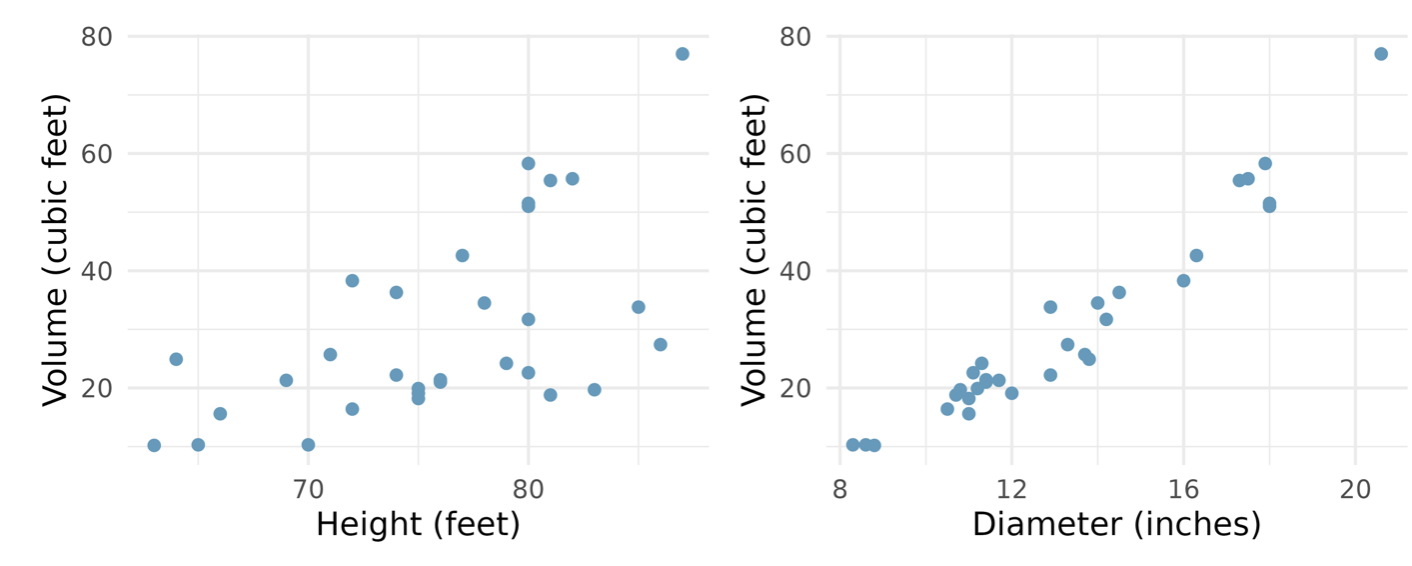
\includegraphics[width=7.29167in,height=\textheight,keepaspectratio]{images/revimg1.png}
\end{center}

\begin{enumerate}
\def\labelenumi{\alph{enumi}.}
\item
  Identify the predictor and response variable in each scatter plot.
  \vspace{2cm}
\item
  Compare the relationships between variables as portrayed in the two
  scatterplots. Be sure to write in full sentences and in context.
  \vspace{4cm}
\item
  The calculated correlation coefficients for the scatter plots are 0.85
  and 0.6. Assign each coefficient to the correct plot (left or right)
  and explain the reasoning for your matching.
\end{enumerate}

\vspace{3cm}

\begin{enumerate}
\def\labelenumi{\alph{enumi}.}
\setcounter{enumi}{3}
\item
  A linear regression using the plot on the left (height vs volume) was
  generated as \(\hat{y}=0.34x+12.1\) where \(y\) is the response and
  \(x\) the predictor.

  \begin{enumerate}
  \def\labelenumii{\roman{enumii})}
  \tightlist
  \item
    Interpret the \emph{slope} and \emph{intercept} of the linear
    regression model line in the context of the data. \vspace{4cm}
  \item
    Use the model to predict the volume of timber produced by a tree
    that is 65 feet tall and 11 inches wide(diameter). Show your work.
    \vspace{3cm}
  \item
    A tree that is 65 feet tall is observed to have a volume of 40 cubic
    feet. Calculate the \emph{residual} for this observation and
    interpret its meaning in the context of the data. \vspace{4cm}
  \item
    Explain why it may not be appropriate to use this model to predict
    the volume of a tree that is 215 feet tall. \vspace{4cm}
  \end{enumerate}

  \clearpage
\end{enumerate}




\end{document}
